\documentclass[13pt]{article}
\usepackage[utf8]{inputenc}
\title{Programmazione Concorrente e Distribuita\\Terza Parte}
\author{Suierica Bogdan Ionut 1008089}
\usepackage{graphicx}
\begin{document}
\maketitle

\begin{figure}[h]
\centering
\includegraphics[width=0.7\linewidth]{../../../../../Dropbox/touslesmemes/RelazioneExtra/img/unipd}
\label{fig:unipd}
\end{figure}

\newpage
\section{Cambiamenti}
In questa sezione verranno descritti i cambiamenti apportati al codice per permettere al programma di essere distribuito tra un server e un client. In particolare la classe \textit{Puzzle} contiene anche una copia dell'insieme non ordinato di Tile che rappresentano il puzzle. La classe \textit{PuzzleToSolve}, in seguito al cambiamento della classe \textit{Puzzle}, implementa l'interfaccia \textit{SolverAlgorithm} con il suo metodo \textit{solve} e si preoccupa solamente della risoluzione del puzzle. Il metodo \textit{solve} dell'interfaccia \textit{SolverAlgorithm} è stato modificato e adesso accetta un parametro di tipo \textit{Puzzle} e ritorno un \textit{Puzzle}.
\begin{figure}[h]
\centering
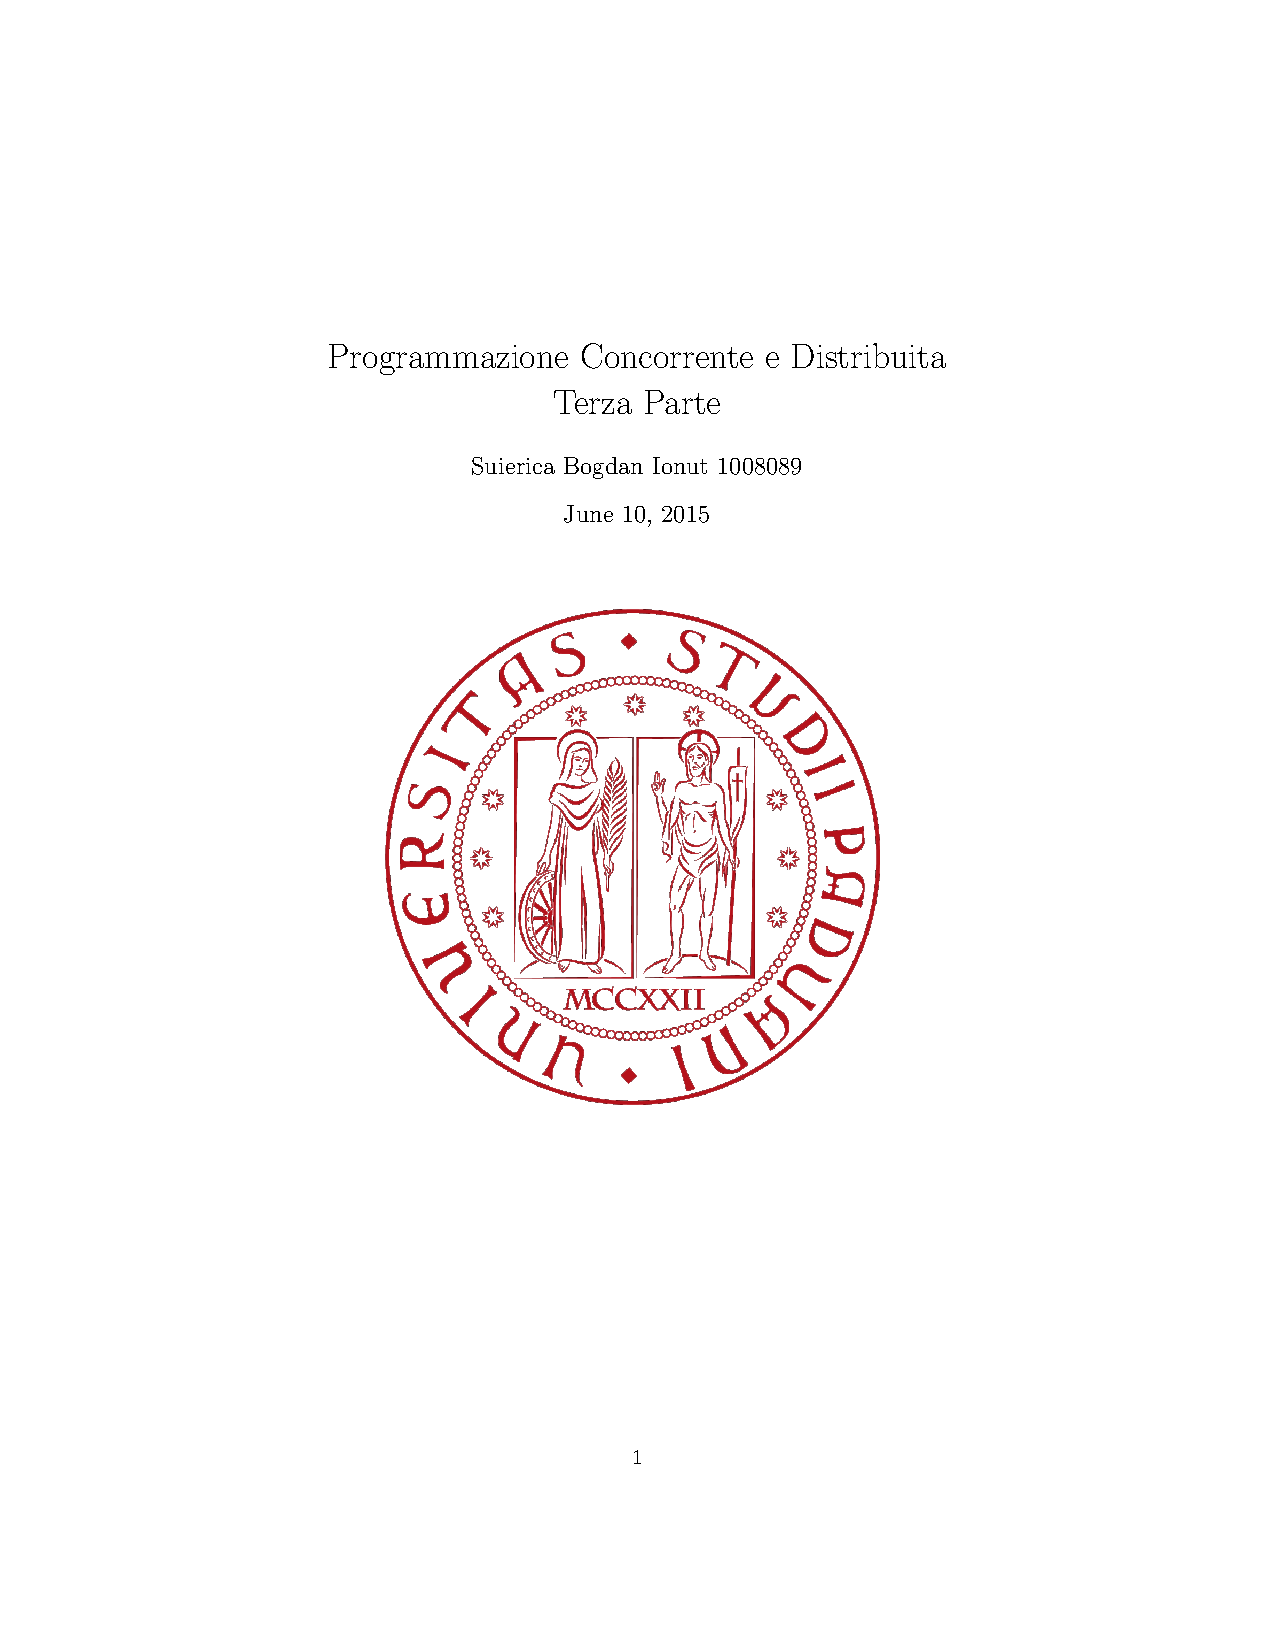
\includegraphics[width=0.9\linewidth]{../../../uml/terzaParte}
\caption{}
\label{fig:terzaParte}
\end{figure}

Come richiesto dalla specifica il client si occupa della gestione dei file di input e di output.\\
Il programma è stato suddiviso in 3 parti. Sono stati quindi individuati 3 package:
\begin{itemize}
	\item \textbf{Server: }il package contiene le classi:
		\begin{itemize}
			\item \textbf{PuzzleToSolve:} la classe definisce l'oggetto remoto implementando l'interfaccia \textit{SolverAlgorithm} con il suo metodo \textit{solve} (che si preoccupa di risolvere il puzzle)  ed estendendo la classe \textit{UnicastRemoteObject}. La classe contiene un costruttore con corpo vuoto che può sollevare un'eccezione di tipo RemoteException;
			\item \textbf{PuzzleSolverServer: }è la classe che definisce il metodo \textit{main}. La classe crea l'istanza dell'oggetto remoto \textit{PuzzleToSolve} e gli associa un nome. Attraverso il metodo \textit{rebind} lo registra nell'RMI registry.
		\end{itemize}
	\item \textbf{Client:}il package contine le classi:
		\begin{itemize}
			\item \textbf{IOReader: }è la classe che si occupa della gestione dei file in input;
			\item \textbf{IOWriter: }è la classe che si occupa della gestione dei file in output;
			\item \textbf{PuzzleSolverClient: }è la classe che contiene il metodo \textit{main}. Il programma client interroga il registro RMI utilizzando il metodo statico \textit{lookup} della classe \textit{Naming}, il quale restituisce un riferimento di tipo \textit{Remote} all'oggetto cercato.Infine invoca il metodo remoto \textit{solve} facendo un downcast al tipo \textit{SolverAlgorithm}.
		\end{itemize}
	\item \textbf{Shared:} il package contiene le classi in comune del server e del client. Le classi \textit{Tile} e \textit{Puzzle} estendono l'interfaccia \textit{Serializable} in quanto gli oggetti vengono passati come parametri e come valori restituiti dal metodo \textit{solve}:
		\begin{itemize}
			\item \textbf{Tile:} rappresenta il singolo pezzo del puzzle;
			\item \textbf{Puzzle:} rappresenta il puzzle;
			\item \textbf{SolverAlgorithm:} rappresenta l'interfaccia remota. L'interfaccia estende l'interfaccia \textit{Remote}. È presente il metodo \textit{solve}, che ha il compito di risolvere il puzzle. Il metodo può sollevare un'eccezione di tipo \textit{RemoteException}.
		\end{itemize}
\end{itemize}

\newpage
\section{Logica di comunicazione client-server}
Per la comunicazione tra un server e un client il programma adotta la libreria RMI il cui scopo è di rendere trasparente al programmatore quasi tutti i dettagli della comunicazione su rete. Essa consenta infatti di invocare un metodo di un oggetto remoto.\\
Per implementare il meccanismo RMI sono richiesti i seguenti punti:
\begin{itemize}
	\item Definizione dell'interfaccia remota \textit{SolverAlgorithm};
	\item Definizione dell'oggetto remote \textit{PuzzleToSolve};
	\item Creazione del server con il compito di creare un'istanza dell'oggetto remoto e registrare il riferimento associandogli una stringa identificativa. La registrazione avviene invocando il metodo statico \textit{rebind} della classe \textit{java.rmi.Naming};
	\item Creazione del client che ha il compito di interrogare il registro RMI utilizzando il metodo statico lookup della classe \textit{java.rmi.Naming}, il quale restituisce un riferimento di tipo \textit{Remote} all'oggetto cercato.
\end{itemize}
La classe \textit{Puzzle e Tile} estondono l'interfaccia \textit{Serializable}. Viene trasmessa quindi una copia.

\newpage
\section{Compilazione}
Dalla root principale è possibile avviare il commando per la compilazione di tutti i file attraverso l'istruzione \textbf{make}. Se si vuole lanciare il programma si devono utilizzare i seguenti script bash:
\begin{itemize}
	\item \textit{sh puzzlesolverserver.sh [nome\_del\_server]} : questo script riceve in input il nome del server. Con il lancio verrà eseguito il commando per avviare il registro rmi e il main del server;
	\item \textit{sh puzzlesolverclient.sh [input\_file][output\_file][nome\_del\_server]} : questo script riceve in input 3 parametri, file in input, file in output e il nome del server. Con il lancio verrà eseguito il main del client. 
\end{itemize}
Prima di procedere con il lancio degli script bash si deve aver compilato.

\end{document}